%%%%%%%%%%%%%%%%%%%%%%%%%%%%%%%%%%%%%%%%
% datoteka diploma-FRI-vzorec.tex
%
% vzorčna datoteka za pisanje diplomskega dela v formatu LaTeX
% na UL Fakulteti za računalništvo in informatiko
%
% na osnovi starejših verzij vkup spravil Franc Solina, maj 2021
% prvo verzijo je leta 2010 pripravil Gašper Fijavž
%
% za upravljanje z literaturo ta vezija uporablja BibLaTeX
%
% svetujemo uporabo Overleaf.com - na tej spletni implementaciji LaTeXa ta vzorec zagotovo pravilno deluje
%

\documentclass[a4paper,12pt,openright]{book}
%\documentclass[a4paper, 12pt, openright, draft]{book}  Nalogo preverite tudi z opcijo draft, ki pokaže, katere vrstice so predolge! Pozor, v draft opciji, se slike ne pokažejo!
 
\usepackage[utf8]{inputenc}   % omogoča uporabo slovenskih črk kodiranih v formatu UTF-8
\usepackage[slovene,english]{babel}    % naloži, med drugim, slovenske delilne vzorce
\usepackage[pdftex]{graphicx}  % omogoča vlaganje slik različnih formatov
\usepackage{fancyhdr}          % poskrbi, na primer, za glave strani
\usepackage{amssymb}           % dodatni matematični simboli
\usepackage{amsmath}           % eqref, npr.
\usepackage{hyperxmp}
\usepackage[hyphens]{url}
\usepackage{csquotes}
\usepackage{listings}
\renewcommand{\lstlistingname}{Izvorna koda}
\lstset{basicstyle=\footnotesize\ttfamily}

\usepackage[pdftex, colorlinks=true,
						citecolor=black, filecolor=black, 
						linkcolor=black, urlcolor=black,
						pdfproducer={LaTeX}, pdfcreator={LaTeX}]{hyperref}

\usepackage{color}
\usepackage{soul}

\usepackage[
backend=biber,
style=numeric,
sorting=nty,
]{biblatex}


\addbibresource{literatura.bib} %Imports bibliography file


%%%%%%%%%%%%%%%%%%%%%%%%%%%%%%%%%%%%%%%%
%	DIPLOMA INFO
%%%%%%%%%%%%%%%%%%%%%%%%%%%%%%%%%%%%%%%%
\newcommand{\ttitle}{Spletna aplikacija za glasbene festivale}
\newcommand{\ttitleEn}{Web application for music festivals}
\newcommand{\tsubject}{\ttitle}
\newcommand{\tsubjectEn}{\ttitleEn}
\newcommand{\tauthor}{Vasja Škarabot}
\newcommand{\tkeywords}{glasba, festival, socialno omrežje, spletna aplikacija}
\newcommand{\tkeywordsEn}{music, festival, social network, web application}

%%%%%%%%%%%%%%%%%%%%%%%%%%%%%%%%%%%%%%%%
%	HYPERREF SETUP
%%%%%%%%%%%%%%%%%%%%%%%%%%%%%%%%%%%%%%%%
\hypersetup{pdftitle={\ttitle}}
\hypersetup{pdfsubject=\ttitleEn}
\hypersetup{pdfauthor={\tauthor}}
\hypersetup{pdfkeywords=\tkeywordsEn}

%%%%%%%%%%%%%%%%%%%%%%%%%%%%%%%%%%%%%%%%
% postavitev strani
%%%%%%%%%%%%%%%%%%%%%%%%%%%%%%%%%%%%%%%%  

\addtolength{\marginparwidth}{-20pt} % robovi za tisk
\addtolength{\oddsidemargin}{40pt}
\addtolength{\evensidemargin}{-40pt}

\renewcommand{\baselinestretch}{1.3} % ustrezen razmik med vrsticami
\setlength{\headheight}{15pt}        % potreben prostor na vrhu
\renewcommand{\chaptermark}[1]%
{\markboth{\MakeUppercase{\thechapter.\ #1}}{}} \renewcommand{\sectionmark}[1]%
{\markright{\MakeUppercase{\thesection.\ #1}}} \renewcommand{\headrulewidth}{0.5pt} \renewcommand{\footrulewidth}{0pt}
\fancyhf{}
\fancyhead[LE,RO]{\sl \thepage} 
%\fancyhead[LO]{\sl \rightmark} \fancyhead[RE]{\sl \leftmark}
\fancyhead[RE]{\sc \tauthor}              % dodal Solina
\fancyhead[LO]{\sc Diplomska naloga}     % dodal Solina


\newcommand{\BibLaTeX}{{\sc Bib}\LaTeX}
\newcommand{\BibTeX}{{\sc Bib}\TeX}

%%%%%%%%%%%%%%%%%%%%%%%%%%%%%%%%%%%%%%%%
% naslovi
%%%%%%%%%%%%%%%%%%%%%%%%%%%%%%%%%%%%%%%%  

\newcommand{\autfont}{\Large}
\newcommand{\titfont}{\LARGE\bf}
\newcommand{\clearemptydoublepage}{\newpage{\pagestyle{empty}\cleardoublepage}}
\setcounter{tocdepth}{1}	      % globina kazala

%%%%%%%%%%%%%%%%%%%%%%%%%%%%%%%%%%%%%%%%
% konstrukti
%%%%%%%%%%%%%%%%%%%%%%%%%%%%%%%%%%%%%%%%  
\newtheorem{izrek}{Izrek}[chapter]
\newtheorem{trditev}{Trditev}[izrek]
\newenvironment{dokaz}{\emph{Dokaz.}\ }{\hspace{\fill}{$\Box$}}


%%%%%%%%%%%%%%%%%%%%%%%%%%%%%%%%%%%%%%%%%%%%%%%%%%%%%%%%%%%%%%%%%%%%%%%%%%%%%%%
%% PDF-A
%%%%%%%%%%%%%%%%%%%%%%%%%%%%%%%%%%%%%%%%%%%%%%%%%%%%%%%%%%%%%%%%%%%%%%%%%%%%%%%

%%%%%%%%%%%%%%%%%%%%%%%%%%%%%%%%%%%%%%%% 
% define medatata
%%%%%%%%%%%%%%%%%%%%%%%%%%%%%%%%%%%%%%%% 
\def\Title{\ttitle}
\def\Author{\tauthor, vs7015@student.uni-lj.si}
\def\Subject{\ttitleEn}
\def\Keywords{\tkeywordsEn}

%%%%%%%%%%%%%%%%%%%%%%%%%%%%%%%%%%%%%%%% 
% \convertDate converts D:20080419103507+02'00' to 2008-04-19T10:35:07+02:00
%%%%%%%%%%%%%%%%%%%%%%%%%%%%%%%%%%%%%%%% 
\def\convertDate{%
    \getYear
}

{\catcode`\D=12
 \gdef\getYear D:#1#2#3#4{\edef\xYear{#1#2#3#4}\getMonth}
}
\def\getMonth#1#2{\edef\xMonth{#1#2}\getDay}
\def\getDay#1#2{\edef\xDay{#1#2}\getHour}
\def\getHour#1#2{\edef\xHour{#1#2}\getMin}
\def\getMin#1#2{\edef\xMin{#1#2}\getSec}
\def\getSec#1#2{\edef\xSec{#1#2}\getTZh}
\def\getTZh +#1#2{\edef\xTZh{#1#2}\getTZm}
\def\getTZm '#1#2'{%
    \edef\xTZm{#1#2}%
    \edef\convDate{\xYear-\xMonth-\xDay T\xHour:\xMin:\xSec+\xTZh:\xTZm}%
}

%\expandafter\convertDate\pdfcreationdate 

%%%%%%%%%%%%%%%%%%%%%%%%%%%%%%%%%%%%%%%%
% get pdftex version string
%%%%%%%%%%%%%%%%%%%%%%%%%%%%%%%%%%%%%%%% 
\newcount\countA
\countA=\pdftexversion
\advance \countA by -100
\def\pdftexVersionStr{pdfTeX-1.\the\countA.\pdftexrevision}


%%%%%%%%%%%%%%%%%%%%%%%%%%%%%%%%%%%%%%%%
% XMP data
%%%%%%%%%%%%%%%%%%%%%%%%%%%%%%%%%%%%%%%%  
\usepackage{xmpincl}
%\includexmp{pdfa-1b}

%%%%%%%%%%%%%%%%%%%%%%%%%%%%%%%%%%%%%%%%
% pdfInfo
%%%%%%%%%%%%%%%%%%%%%%%%%%%%%%%%%%%%%%%%  
\pdfinfo{%
    /Title    (\ttitle)
    /Author   (\tauthor, vs7015@student.uni-lj.si)
    /Subject  (\ttitleEn)
    /Keywords (\tkeywordsEn)
    /ModDate  (\pdfcreationdate)
    /Trapped  /False
}

%%%%%%%%%%%%%%%%%%%%%%%%%%%%%%%%%%%%%%%%
% znaki za copyright stran
%%%%%%%%%%%%%%%%%%%%%%%%%%%%%%%%%%%%%%%%  

\newcommand{\CcImageCc}[1]{%
	
\includegraphics[scale=#1]{cc_cc_30.pdf}%
}
\newcommand{\CcImageBy}[1]{%
	
\includegraphics[scale=#1]{cc_by_30.pdf}%
}
\newcommand{\CcImageSa}[1]{%
	
\includegraphics[scale=#1]{cc_sa_30.pdf}%
}

%%%%%%%%%%%%%%%%%%%%%%%%%%%%%%%%%%%%%%%%%%%%%%%%%%%%%%%%%%%%%%%%%%%%%%%%%%%%%%%
%%%%%%%%%%%%%%%%%%%%%%%%%%%%%%%%%%%%%%%%%%%%%%%%%%%%%%%%%%%%%%%%%%%%%%%%%%%%%%%

\begin{document}
\selectlanguage{slovene}
\frontmatter
\setcounter{page}{1} %
\renewcommand{\thepage}{}       % preprečimo težave s številkami strani v kazalu

%%%%%%%%%%%%%%%%%%%%%%%%%%%%%%%%%%%%%%%%
%naslovnica
 \thispagestyle{empty}%
   \begin{center}
    {\large\sc Univerza v Ljubljani\\%
%      Fakulteta za elektrotehniko\\% za študijski program Multimedija
%      Fakulteta za upravo\\% za študijski program Upravna informatika
      Fakulteta za računalništvo in informatiko\\%
%      Fakulteta za matematiko in fiziko\\% za študijski program Računalništvo in matematika
     }
    \vskip 10em%
    {\autfont \tauthor\par}%
    {\titfont \ttitle \par}%
    {\vskip 3em \textsc{DIPLOMSKO DELO\\[5mm]         % dodal Solina za ostale študijske programe
    VISOKOŠOLSKI STROKOVNI ŠTUDIJSKI PROGRAM\\ PRVE STOPNJE\\ RAČUNALNIŠTVO IN INFORMATIKA}\par}%
%     UNIVERZITETNI  ŠTUDIJSKI PROGRAM\\ PRVE STOPNJE\\ RAČUNALNIŠTVO IN INFORMATIKA}\par}%
%    INTERDISCIPLINARNI UNIVERZITETNI\\ ŠTUDIJSKI PROGRAM PRVE STOPNJE\\ MULTIMEDIJA}\par}%
%    INTERDISCIPLINARNI UNIVERZITETNI\\ ŠTUDIJSKI PROGRAM PRVE STOPNJE\\ UPRAVNA INFORMATIKA}\par}%
%    INTERDISCIPLINARNI UNIVERZITETNI\\ ŠTUDIJSKI PROGRAM PRVE STOPNJE\\ RAČUNALNIŠTVO IN MATEMATIKA}\par}%
    \vfill\null%
% izberite pravi habilitacijski naziv mentorja!
    {\large \textsc{Mentor}: viš. pred. dr. Aljaž Zrnec\par}%
    {\vskip 2em \large Ljubljana, \the\year \par}%
\end{center}
% prazna stran
%\clearemptydoublepage      
% izjava o licencah itd. se izpiše na hrbtni strani naslovnice

%%%%%%%%%%%%%%%%%%%%%%%%%%%%%%%%%%%%%%%%
%copyright stran
%%%%%%%%%%%%%%%%%%%%%%%%%%%%%%%%%%%%%%%%
\newpage
\thispagestyle{empty}

\vspace*{5cm}
{\small \noindent
To delo je ponujeno pod licenco \textit{Creative Commons Priznanje avtorstva-Deljenje pod enakimi pogoji 2.5 Slovenija} (ali novej\v so razli\v cico).
To pomeni, da se tako besedilo, slike, grafi in druge sestavine dela kot tudi rezultati diplomskega dela lahko prosto distribuirajo,
reproducirajo, uporabljajo, priobčujejo javnosti in predelujejo, pod pogojem, da se jasno in vidno navede avtorja in naslov tega
dela in da se v primeru spremembe, preoblikovanja ali uporabe tega dela v svojem delu, lahko distribuira predelava le pod
licenco, ki je enaka tej.
Podrobnosti licence so dostopne na spletni strani \href{http://creativecommons.si}{creativecommons.si} ali na Inštitutu za
intelektualno lastnino, Streliška 1, 1000 Ljubljana.

\vspace*{1cm}
\begin{center}% 0.66 / 0.89 = 0.741573033707865
\CcImageCc{0.741573033707865}\hspace*{1ex}\CcImageBy{1}\hspace*{1ex}\CcImageSa{1}%
\end{center}
}

\vspace*{1cm}
{\small \noindent
Izvorna koda diplomskega dela, njeni rezultati in v ta namen razvita programska oprema je ponujena pod licenco GNU General Public License,
različica 3 (ali novejša). To pomeni, da se lahko prosto distribuira in/ali predeluje pod njenimi pogoji.
Podrobnosti licence so dostopne na spletni strani \url{http://www.gnu.org/licenses/}.
}

\vfill
\begin{center} 
\ \\ \vfill
{\em
Besedilo je oblikovano z urejevalnikom besedil \LaTeX.}
\end{center}

% prazna stran
\clearemptydoublepage

%%%%%%%%%%%%%%%%%%%%%%%%%%%%%%%%%%%%%%%%
% stran 3 med uvodnimi listi
\thispagestyle{empty}
\
\vfill

\bigskip
\noindent\textbf{Kandidat:} Vasja Škarabot \\
\noindent\textbf{Naslov:} Spletna aplikacija za glasbene festivale\\
% vstavite ustrezen naziv študijskega programa!
\noindent\textbf{Vrsta naloge:} Diplomska naloga na visokošolskem programu prve stopnje Računalništvo in informatika \\
% izberite pravi habilitacijski naziv mentorja!
\noindent\textbf{Mentor:} viš. pred. dr. Aljaž Zrnec\\

\bigskip
\noindent\textbf{Opis:}\\
Besedilo teme diplomskega dela študent prepiše iz študijskega informacijskega sistema, kamor ga je vnesel mentor. 
V nekaj stavkih bo opisal, kaj pričakuje od kandidatovega diplomskega dela. 
Kaj so cilji, kakšne metode naj uporabi, morda bo zapisal tudi ključno literaturo.

\bigskip
\noindent\textbf{Title:} Web application for music festivals

\bigskip
\noindent\textbf{Description:}\\
opis diplome v angleščini

\vfill



\vspace{2cm}

% prazna stran
\clearemptydoublepage

% zahvala
\thispagestyle{empty}\mbox{}\vfill\null\it%
\noindent
Na tem mestu zapišite, komu se zahvaljujete za pomoč pri izdelavi diplomske naloge oziroma pri vašem študiju nasploh. Pazite, da ne boste koga pozabili. Utegnil vam bo zameriti. Temu se da izogniti tako, da celotno zahvalo izpustite.
\rm\normalfont

% prazna stran
\clearemptydoublepage


%%%%%%%%%%%%%%%%%%%%%%%%%%%%%%%%%%%%%%%%
% kazalo
\pagestyle{empty}
\def\thepage{}% preprečimo težave s številkami strani v kazalu
\tableofcontents{}


% prazna stran
\clearemptydoublepage

%%%%%%%%%%%%%%%%%%%%%%%%%%%%%%%%%%%%%%%%
% seznam kratic

\chapter*{Seznam uporabljenih kratic}

\noindent\begin{tabular}{p{0.11\textwidth}|p{.39\textwidth}|p{.39\textwidth}}    % po potrebi razširi prvo kolono tabele na račun drugih dveh!
  {\bf kratica} & {\bf angleško}                              & {\bf slovensko} \\ \hline
  {\bf API}      & application programming interface               & aplikacijski programski vmesnik \\
  {\bf CRUD}    & create, read, update and delete & ustvarjanje, branje, posodabljanje in brisanje \\
  {\bf DBMS} & database management system & sistem za upravljanje podatkovnih baz \\
  {\bf ORM}  & object-relational mapping & objektno-relacijsko preslikovanje \\
  {\bf SSR}  & server-side rendering & upodabljanje na strani stre-žnika \\
  {\bf SVM}   & support vector machine              & metoda podpornih vektorjev \\
  {\bf MVC}  & model-view-controller & model-pogled-kontroler \\
  {\bf MVT}   & model-view-template  & model-pogled-predloga \\
%  \dots & \dots & \dots \\
\end{tabular}


% prazna stran
\clearemptydoublepage

%%%%%%%%%%%%%%%%%%%%%%%%%%%%%%%%%%%%%%%%
% povzetek
\phantomsection
\addcontentsline{toc}{chapter}{Povzetek}
\chapter*{Povzetek}

\noindent\textbf{Naslov:} \ttitle
\bigskip

\noindent\textbf{Avtor:} \tauthor
\bigskip

%\noindent\textbf{Povzetek:} 
\noindent 
Diplomska naloga predstavlja razvoj in implementacijo spletne aplikacije za glasbene festivale. Glavni namen aplikacije je, uporabnikom olajšati
dostop do vseh pomembnih informacij, ter jim omogočiti medsebojno komunikacijo in preko le te graditi skupnosti s pomočjo forumov in klepetov. 

Spletna aplikacija uporabniku omogoča pregled nad festivali, vključno z iskanjem prenočišč v bližini ter navodili za pot do prizorišča, forum na katerem lahko uporabniki
objavljajo novice, delijo nasvete ter postavljajo morebitna vprašanja, ki se jim porajajo, ter klepeti, katere lahko uporabniki uporabijo z namenom razpravljanja in dogovarjanja za skupni obisk. 

Za implementacijo čelnega dela smo uporabili ogrodje Nuxt.js, za zaledni del pa Django z razširitvijo REST Framework in podatkovno bazo PostgreSQL. Vse skupaj poganjamo v Dockerju.
Zemljevidi so implementirani s pomočjo platforme Mapbox, realnočasovno komunikacijo v klepetih omogoča Pusher, slike pa shranjujemo s pomočjo Firebase shrambe.

\bigskip

\noindent\textbf{Ključne besede:} \tkeywords.
% prazna stran
\clearemptydoublepage

%%%%%%%%%%%%%%%%%%%%%%%%%%%%%%%%%%%%%%%%
% abstract
\phantomsection
\selectlanguage{english}
\addcontentsline{toc}{chapter}{Abstract}
\chapter*{Abstract}

\noindent\textbf{Title:} \ttitleEn
\bigskip

\noindent\textbf{Author:} \tauthor
\bigskip

%\noindent\textbf{Abstract:} 
\noindent 
The thesis presents the development and implementation of a web application for music festivals. The main purpose of the application is to make it easier for users
access to all relevant information, and to allow users to communicate with each other and build communities through forums and chats. 

The web application provides the user with an overview of the festivals, including a search for nearby accommodation and directions to the venue, a forum where users can
post news, share tips and ask any questions they may have, and chat rooms which users can use to discuss and arrange to visit together. 

For the front-end implementation, we used the Nuxt.js framework, and for the back-end we used Django with the REST Framework extension and the PostgreSQL database. 
We run everything inside Docker containers. Maps are implemented using the Mapbox platform, real-time communication in chats is enabled by Pusher, and images are stored using the Firebase Storage.

\bigskip

\noindent\textbf{Keywords:} \tkeywordsEn.
\selectlanguage{slovene}
% prazna stran
\clearemptydoublepage

%%%%%%%%%%%%%%%%%%%%%%%%%%%%%%%%%%%%%%%%
\mainmatter
\setcounter{page}{1}
\pagestyle{fancy}

\chapter{Uvod}
\section{Motivacija}
Veliko ljudi vsako leto obišče kakšen glasbeni festival.
Pridobivanje informacij za načrtovanje samega obiska festivala pa lahko kar hitro postane nadležno, in lahko hitro pokvari izkušnjo še pred samim festivalom.
Običajno uporabnik najprej izbere glasbeni festival, ki se ga bo udeležil.
Ponavadi to stori na podlagi različnih dejavnikov, kot so lokacija, datumi in žanri, pri končni izbiri pa veliko pripomorejo tudi nasveti ostalih ljudi, predvsem tistih ki so v preteklosti že obiskali izbrani festival.
Problem pri tem pa je, da je potrebno vse izmed naštetih informacij iskati po različnih spletnih straneh saj rešitve, ki bi ponujala vse to na enem mestu ni. 
Zato bi bilo smiselno implementirati rešitev, ki bo uporabnikom omogočila vpogled v vse na enem mestu, s tem da si uporabniki pomagajo med sabo.

\section{Cilji}
Cilj diplomske naloge je torej razviti sodobno spletno aplikacijo, ki bo uporabnikom olajšala iskanje glasbenih festivalov in udeležbo na njih.
Želimo tudi skrajšati proces planiranja tako, da uporabniku omogočimo iskanje poti do glasbenega festivala, ter bližnjih prenočišč.
Za vsa vprašanja, ki se uporabniku pojavljajo bodo na voljo forumi, na katerih bodo uporabniki ustvarjali skupnosti za glasbene festivale.
Želimo pa tudi vzpodbuditi interakcijo med obiskovalci festivalov, ki morda potujejo sami ali pa tistih, ki so že na prizorišču in s tem izboljšati festivalsko izkušnjo, za kar bomo razvili sistem klepetov.

\section{Struktura diplomske naloge}
Diplomsko nalogo sestavlja 7 poglavij.
Najprej bomo preverili obstoječe rešitve, ter njihove pomankljivosti, pa tudi morebitne prednosti.
Za tem bo sledil zajem zahtev, kjer bomo opisali funkcionalnosti sistema, ter predstavili diagram primerov uporabe.
Sledilo bo poglavje v katerem bomo predstavili uporabljene tehnologije in orodja, ter razlogi zakaj smo se odločili za uporabo teh.
V petem poglavju bomo predstavili razvoj rešitve, v katerem bomo vključili samo arhitekturo aplikacije, potem načrtovanje podatkovne baze, ter implementacija čelnega in zalednega dela.
V naslednjem poglavju bomo nato predstavili še našo končno rešitev s pomočjo slik uporabniškega vmesnika, ter opisom delovanja vseh pomembnejših funkcionalnosti.
V zaključku, pa bomo povzeli našo nalogo, ter podali nekaj mogočih izboljšav v nadaljnjem razvoju.

\chapter{Obstoječe rešitve}
Na trgu trenutno ni nobene podobne rešitve, zaradi česar se obiskovalci festivalov poslužujejo različnih aplikacij in spletnih strani. 
Za postavljanje vprašanj sta to običajno Reddit ali pa Tripadvisor. Ti rešitvi nista primarno namenjeni glasbenim festivalom, 
zato težko najdemo koristne podatke, saj vsebujeta le forume za večje festivale.
Poleg tega mora vsak uporabljati več aplikacij za različne namene in zato nimamo vsega na eni platformi. Uporabnik mora tako npr. za iskanje informacij o festivalu najprej na spletno stran festivala,
nato prebira različne forume (Reddit, Tripadvisor), zraven tega še išče prenočišča na Bookingu, potem pa se še na tretji platformi z ostalimi pogovarja/dogovarja (npr. Messenger).
V tem poglavju bodo opisane naštete alternative, njihove prednosti in slabosti.

\section{Tripadvisor}
Tripadvisor je spletna platforma za iskanje prenočišč~\cite{tripadvisor}. Je ena večjih platform namenjenih planiranju potovanj, ki uporabnikom omogoča tudi podajanje kritik in ocen.

\begin{itemize}
    \item \textbf{Prednosti}:
        \begin{itemize}
            \item Velik nabor uporabnikov in posledično kritik in ocen za prenočišča in razne dogodke.
            \item Širok nabor funkcionalnosti. Poleg osnovnih funkcionalnosti še orodja za načrtovanje poti, vodniki in priporočila.
        \end{itemize}
    \item \textbf{Slabosti}:
        \begin{itemize}
            \item Vsebuje le najpopularnejše festivale.
            \item Ocene bolj osredotočene na nastanitve in potovanje kot na sam festival.
            \item Ne vsebuje nekaterih pomembnih informacij, kot so datumi, informacije o cenah in izvajalcih.
            \item Uporabnik lahko z ostalimi uporabniki komunicira le posredno preko foruma. Za neposredno komunikacijo se mora poslužiti drugih platform.
        \end{itemize}
\end{itemize}

\section{Reddit}
Reddit je forumsko socialno omrežje, kjer lahko uporabniki objavljajo, ostali pa nato te objave komentirajo in glasujejo~\cite{reddit}. Objave so razvrščene v podstrani imenovane subredditi oz. skupnosti.
Na Redditu najdemo skupnosti za nekatere glasbene festivale, kjer se uporabniki obveščajo o novicah o festivalu in podajajo različna vprašanja. Je pa teh skupnosti precej malo, še tiste ki so, 
pa so po večini skupnosti največjih glasbenih festivalov na svetu (Coachella, Tomorrowland, UMF).

\begin{itemize}
    \item \textbf{Prednosti}:
        \begin{itemize}
            \item Pri večjih festivalih ogromen nabor vprašanj, razprav, nasvetov in novic.
            \item Možnost realnočasovne komunikacije z ostalimi.
        \end{itemize}
    \item \textbf{Slabosti}:
        \begin{itemize}
            \item Večino osnovnih informacij mora uporabnik pridobiti na ostalih straneh.
            \item Težko je najti skupnosti, ki niso namenjene le največjim festivalom.
            \item Čeprav lahko uporabniki komunicirajo v realnem času, lahko to počnejo le v privatnih skupinah, ki niso del subredditov.
        \end{itemize}
\end{itemize}

\section{Woov}
Woov je namenska aplikacija za obiskovalce glasbenih festivalov~\cite{woov}. Povezani so z več kot 1000 dogodki po 40 državah, uporabnikom pa omogočajo vpogled v časovnice, zemljevid prizorišč in komunikacijo z ostalimi uporabniki.
Namen aplikacije je pomagati obiskovalcem, ki so že na prizorišču.

\begin{itemize}
    \item \textbf{Prednosti}:
        \begin{itemize}
            \item Uporabniki lahko aplikacijo prenesejo na telefon.
            \item Pomembne informacije kot so datumi, prizorišče, nastopajoči izvajalci.
            \item Uporabniki si lahko pomagajo z zemljevidom, ki vključuje lokacije stojnic, wc-jev, odrov in polnilnih postaj.
            \item Realnočasovna komunikacija.
        \end{itemize}
    \item \textbf{Slabosti}:
        \begin{itemize}
            \item Dogodki so običajno dodani nekaj dni pred začetkom festivala. Posledično si uporabnik za planiranje ne more dosti pomagati.
            \item Aplikacija včasih deluje nelogična za nove uporabnike, saj so nekatere funkcionalnosti precej skrite.
            \item Uporabniki ne morejo podati svojih mnenj.
            \item Aplikaciji lahko prispevajo le partnerji. To ni nujno slabo, vendar omeji aplikacije le na določene festivale.
        \end{itemize}
\end{itemize}

% NOVO POGLAVJE
\chapter{Zajem zahtev}
Preden smo sploh začeli z načrtovanjem podatkovne baze in kodiranjem, je bilo potrebno definirati vse naloge, ki jih bo sistem opravljal.
S tem smo si zadali načrt in ogrodje, kateremu smo pri razvoju nato sledili.
Z dobro definicijo zahtev smo dosegli to, da smo zmanjšali verjetnost pomembnih sprememb med razvojem, s čimer smo prihranili čas in trud.

\section{Funkcionalnosti sistema}
Naša aplikacija mora uporabniku omogočiti:
\begin{itemize}
    \item Registracijo in prijavo.
    \item Pregled glasbenih festivalov z možnostjo iskanja in filtriranja.
    \item Dodajanje novih festivalov in dodeljevanje moderatorskih pravic.
    \item Pregled podrobnosti glasbenih festivalov, vključno z datumi, žanri in povezavo do uradne spletne strani.
    \item Zemljevid z lokacijo glasbenega festivala, ki se lahko razširi v navodila za pot.
    \item Iskanje prenočišč v okolici glasbenega festivala glede na podane parametre.
    \item Branje objav in možnost filtriranja in iskanja na forumu za določen festival.
    \item Objavljanje na forumih.
    \item Všečkanje in komentiranje objav.
    \item Dodajanje javnih klepetov za festivale.
    \item Pošiljanje sporočil v klepetih.
    \item Naročanje na obvestila za nova sporočila.
\end{itemize}

Moderatorjem pa povrh vsega še:
\begin{itemize}
    \item Urejajanje podatkov za svoje festivale.
    \item Brisanje objav in komentarjev z namenom odstranjevanja neprimerne vsebine.
\end{itemize}

\section{Diagram primerov uporabe}
Na Sliki~\ref{usecase} je prikazan diagram primerov uporabe za našo aplikacijo. 
V diagramu nastopata 2 akterja in sicer Uporabnik in Moderator.
Iz diagrama je razvidno, kaj lahko oba tipa uporabnikov počneta v aplikaciji.
Podrobnejši opis vseh funkcionalnosti pa bomo predstavili v poglavju~\ref{UI}.

\begin{figure}[p] % OPTIONS h-here, t-top, b-bottom, p-page
\begin{center}
    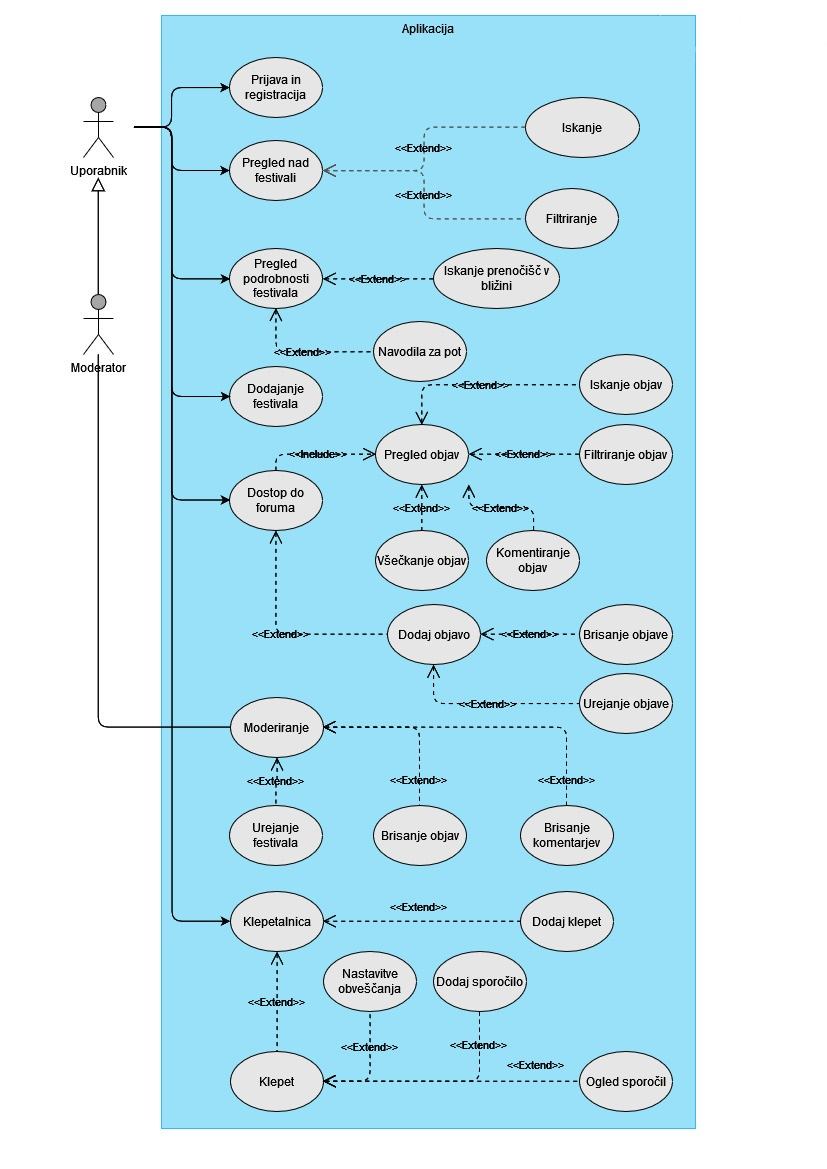
\includegraphics[width=0.99\textwidth]{img/UseCase}
\end{center}
\caption{Diagram primerov uporabe.}
\label{usecase}
\end{figure}

% NOVO POGLAVJE
\chapter{Uporabljene tehnologije in orodja}
Odločili smo se za uporabo modernih, dobro poznanih in pogosto uporabljenih tehnologij in orodij.
Tako smo za čelni del uporabili Nuxt~\cite{nuxtintro}, ki temelji na ogrodju Vue.js~\cite{vuejs}.
Zaledni del smo implementirali z uporabo Djanga~\cite{django} s knjižnico Django REST Framework~\cite{drf}, ki nam je močno olajšala razvoj API vmesnika in upravljanje s podatkovno bazo.
Za podatkovno bazo smo uporabili PostgreSQL~\cite{postgre}.
Pri tem smo podatkovno bazo ter Django strežnik poganjali v Dockerju~\cite{docker}.
Realnočasovno komunikacijo smo omogočili s pomočjo Pusher Channels~\cite{pusher}, zemljevide in navodila za pot pa smo osnovali na platformi Mapbox~\cite{mapbox}.
Vse te tehnologije in orodja, ter njihov namen in uporabo v naši rešitvi smo podrobneje predstavili v naslednjem poglavju.

Sicer, pa smo poleg omenjenih glavnih tehnologij še Vuetify.js za oblikovanje spletne strani~\cite{vuetify},
Git \cite{git} in GitHub \cite{github} za nadzor različic, Firebase Storage~\cite{firebase} za shranjevanje slik in Visual Studio Code~\cite{vscode} za urejanje kode.
Poleg tega smo uporabili še nekaj Python knjižnic, med njimi BeautifulSoup4~\cite{bs4} za strganje podatkov iz Bookinga~\cite{bookingapi}, ter Djoser~\cite{djoser}, ki ponuja vnaprej definirane končne točke za registracijo, prijavo, odjavo in aktivacijo uporabniškega računa. 

\section{Nuxt.js}
Nuxt.js (na kratko Nuxt) je brezplačno odprtokodno orodje za razvoj čelnega dela spletnih aplikacij z Vue.js.
V naši aplikaciji smo ga uporabili zato, ker omogoča hiter, enostaven, predvsem pa učinkovit razvoj aplikacij. 

Poleg tega Nuxt nudi tudi možnosti SSR, ki omogoča hitrejše čase nalaganja strani in optimizacijo spletnih strani.
Pri tem strežnik po začetni zahtevi odjemalca pošlje v celoti renderirano stran nazaj odjemalcu.
JavaScript na strani odjemalca nato omogoči, da statična stran postane interaktivna Vue.js aplikacija (hidracija)~\cite{hydration}.

Ena večjih prednosti uporabe je tudi enostavna konfiguracija poti na spletni strani, saj Nuxt samodejno razbere strukturo glede na vsebino mape \textit{pages/}. 
V Vue.js npr. je za vsako novo dodano stran to potrebno storiti ročno.

\section{Django in Django REST Framework}
Django je Python ogrodje za razvoj spletnih aplikacij, ustvarjeno z namenom da uporabniku omogoči hiter razvoj, saj vsebuje širok nabor orodij, ki poskrbijo za pogosto uporabljena opravila spletnega razvoja (avtentikacija, administracija, upravljanje z podatkovno bazo...).
Temelji na vzorcu MVT, ki je v osnovi zelo podoben bolj znanemu MVC, pri čemer~\cite{mvt}:
\begin{itemize}
    \item Model (M) skrbi za podatke in vzdržuje povezavo s podatkovno bazo.
    \item Pogled (View - V) sprejema zahtevke in vrača odgovore.
    \item Predloga (Template - T) pa definira strukturo in postavitev strani. V naši aplikaciji smo predlogo modela MVT nadomestili z uporabo Nuxt.js.
\end{itemize}

Django REST Framework je razširitev za Django, posebej namenjena za gradnjo RESTful APIjev.
V naši aplikaciji je bil uporabljen predvsem zaradi enostavnega dela s podatkovno bazo, enostavne serializacije podatkov in že vnaprej pripravljenih pogledov za nekatere osnovne CRUD operacije, ki jih z lahkoto lahko priredimo za naše namene.
Poleg tega omogoča tudi enostavno pisanje pravic za dostop do API končnih točk.

\section{PostgreSQL}
Za podatkovno bazo smo uporabili PostgreSQL.
PostgreSQL je zmogljiv odprtokoden objektno-relacijski DBMS (sistem za upravljanje s podatkovnimi bazami).
Kljub temu, da je odprtokoden se lahko kosa z ostalimi ponudniki, kot sta npr. Oracle in MySQL.
Prav zaradi stroškov, se zelo pogosto uporablja v različnih startupih in za v raziskovalne namene~\cite{juba2015learning}.

\section{Pusher Channels}
Realnočasovno komunikacijo v klepetih smo zagotovili s pomočjo storitve Pusher Channels.
Pusher Channels deluje na tehnologiji WebSockets, ki omogoča vztrajne TCP povezave med strežnikom in odjemalcem.
S tem lahko strežnik in odjemalec dosežeta takojšnjo izmenjavo sporočil na zelo učinkovit način z zelo majhno zakasnitvijo, brez potrebe po tem, da bi odjemalec moral ponovno poslati zahtevo za prejem podatkov~\cite{websockets}.

Pusher Channelsi delujejo na modelu objavi/naroči.
To pomeni, da se aplikacije lahko naročajo na kanale v sistemu.
Ko pride do sprememb, sistem objavi spremembo v ta isti kanal in vse aplikacije, ki so naročene na ta kanal, so potem obveščene~\cite{pusher}.

\section{Mapbox}
Mapbox je spletna platforma, ki razvijalcem ponuja širok nabor orodij za delo z zemljevidi.
Podatke črpa iz različnih virov, med drugim tudi iz MapStreetBoxa in NASE. 
V naši aplikaciji smo uporabili večino glavnih storitev, ki jih omogoča in sicer~\cite{mapboxservices}:
\begin{itemize}
    \item \textbf{Mapbox Maps}, ki omogoča prikaz zemljevidov z lokacijami.
    \item \textbf{Mapbox Directions API}, ki omogoča iskanje poti. Naši aplikaciji vrača vse podatke za pot od vnešene lokacije do festivala.
    \item \textbf{Geocoding API}, ki spreminja geografske koordinate v naslove in obratno. V naši aplikaciji je uporabljen, da koordinate zemljepisne širine in dolžine pretvori v človeku prijazno predstavitev.
    \item \textbf{Mapbox Search Box}, ki omogoča iskanje lokacij. V naši aplikaciji je uporabljen za iskanje začetnih lokacij pri navigaciji in za interaktivno iskanje po zemljevidu.
\end{itemize}

\section{Docker}
Docker je platforma, ki omogoča ustvarjanje, izvajanje in nameščanje aplikacij v kontejnerjih/vsebnikih.
Temu procesu pravimo kontejnerizacija.
Pri kontejnerizaciji zapakiramo programsko kodo s knjižnicami operacijskega sistema in odvisnostmi, ki so potrebne za izvajanje kode v lahko, izvedljivo datoteko, ki se lahko enako izvaja na kateri koli infrastrukturi~\cite{containerization}.
Prednosti uporabe Dockerja je veliko, v našem primeru pa smo Docker uporabili predvsem zaradi izolacije okolja in lahke prenosljivosti.
V Dockerju smo poganjali Django aplikacijo ter podatkovno bazo.

% NOVO POGLAVJE
\chapter{Razvoj rešitve}
V tem poglavju bomo predstavili celoten proces razvoja naše rešitve, od začetnega načrtovanja arhitekture in podatkovne baze, do končne rešitve.
Pri tem se bomo posvetili predvsem implementaciji pomembnejših funkcionalnosti sistema.

\section{Arhitektura aplikacije}
Spletna aplikacija je sestavljena iz čelnega dela implementiranega z Nuxt.js, ki pridobiva podatke preko APIja implementiranega v Django REST Frameworku.
V zalednem delu imamo Django REST Framework, ki je povezan s Pusher Channels, da se ob vsakem dodanem sporočilu v klepetih takoj pošlje obvestilo na čelni del aplikacije in prikaže uporabniku.
Django pa s svojo implementacijo ORM skrbi za upravljanje s podatkovnimi modeli in poizvedbami.
Poleg tega Django pridobiva podatke o prenočiščih iz spletne strani Booking.com s pomočjo skripte za strganje podatkov.
Na Sliki \ref{architecture} je prikazana arhitektura naše rešitve.

\begin{figure}[htb] % OPTIONS h-here, t-top, b-bottom, p-page
\begin{center}
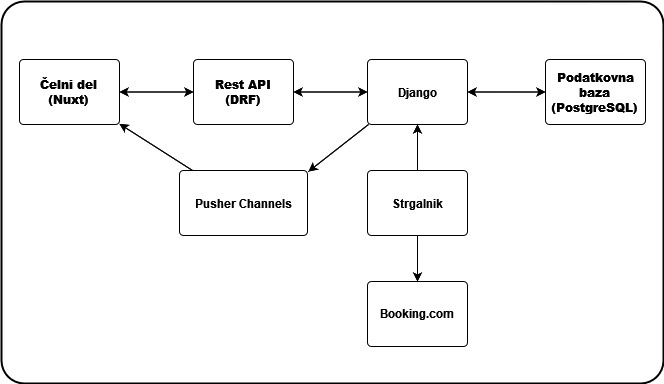
\includegraphics[width=\textwidth]{img/Architecture}
\end{center}
\caption{Arhitektura razvite rešitve.}
\label{architecture}
\end{figure}

\section{Podatkovni model}
Podatkovni model lahko za lažjo predstavo razdelimo na štiri dele:
\begin{itemize}
    \item \textbf{Tabela uporabnika}
        \begin{itemize}
            \item \textbf{CustomUser} vsebuje uporabniško ime, e-pošto, geslo in ostale pomembne podatke uporabnika. Lahko vsebuje povezave na tabele \textit{Comment}, \textit{Message}, \textit{Post}, ter vmesne tabele, ki služijo vše-čkanju objav in komentarjev.
        \end{itemize}
    \item \textbf{Tabele za glasbene festivale}
        \begin{itemize}
            \item \textbf{Festival} predstavlja glasbeni festival in med drugim vsebuje podatke o imenu, opisu, povezavi do spletne strani, lokaciji in datumih izvedbe. Festival ima lahko tudi določen klepet (\textit{Chat}) in objave (\textit{Post}), ki tvorijo forum.
            \item \textbf{UserFestival} predstavlja vmesno tabelo med \textit{CustomUser} in \textit{Festival}. Uporabniku omogoča, da postane moderator glasbenega festivala.
            \item \textbf{UserFavouriteFestival} tudi predstavlja vmesno tabelo med \textit{CustomUser} in \textit{Festival}. Uporabniku omogoča dodajanje glasbenih festivalov med priljubljene.
        \end{itemize}
    \item \textbf{Tabele za forum}
        \begin{itemize}
            \item \textbf{Post} vsebuje vse podatke objav, kot so naslov, vsebina in čas objave. Vsebuje tudi festival \textit{Festival} in uporabnika \textit{CustomUser}.  
            \item \textbf{PostLikedBy} predstavlja vmesno tabelo med uporabnikom in objavo. Tabela je namenjena temu, da lahko uporabnik všečka objave.
            \item \textbf{PostDislikedBy} podobno kot \textit{PostLikedBy} predstavlja vmesno tabelo med uporabnikom in objavo. Namenjena je temu, da lahko uporabnik objave označi z 'ni mi všeč'.
            \item \textbf{Comment} predstavlja komentar objave in vsebuje podatke o vsebini, času in morebitnem izbrisu objave. Komentar ima tudi pripadajočo objavo, avtorja in všečke. Da smo lahko implementirali gnezdenje komentarjev smo uporabili polje \textit{parent} - tuji ključ, ki se sklicuje na isto tabelo.
            \item \textbf{CommentLikedBy} predstavlja vmesno tabelo med uporabnikom in komentarjem. Tabela je namenjena temu, da lahko uporabnik všečka komentarje.
            \item \textbf{CommentDislikedBy} podobno kot \textit{CommentLikedBy} predstavlja vmesno tabelo med uporabnikom in komentarjem. Namenjena je temu, da lahko uporabnik komentarje označi z 'ni mi všeč'.
        \end{itemize}
    \item \textbf{Tabele za klepete}
        \begin{itemize}
            \item \textbf{Chat} vsebuje podatek o imenu klepeta in festival, kateremu klepet pripada.
            \item \textbf{Message} vsebuje čas in vsebino sporočila (tekst in slika), ter podatek o avtorju sporočila, pripadajočem klepetu in vsa obvestila povezana s sporočilom.
            \item \textbf{Notification} vsebuje podatke o času obvestila, statusu, ki pove ali je sporočilo bilo prebrano, ter podatke o prejemniku in klepetu v katerem je bilo sporočilo poslano, pa tudi sporočilo, na katerega se obvestilo navezuje.
            \item \textbf{NotifiedUsers} je vmesna tabela med uporabnikom in klepetom. Uporabnikom omogoča, da se lahko prijavijo in odjavijo na obve-ščanje za izbrani klepet.
        \end{itemize}
\end{itemize}

Na sliki \ref{baza} je prikazan celoten podatkovni model.

\begin{figure}[p] % OPTIONS h-here, t-top, b-bottom, p-page
\begin{center}
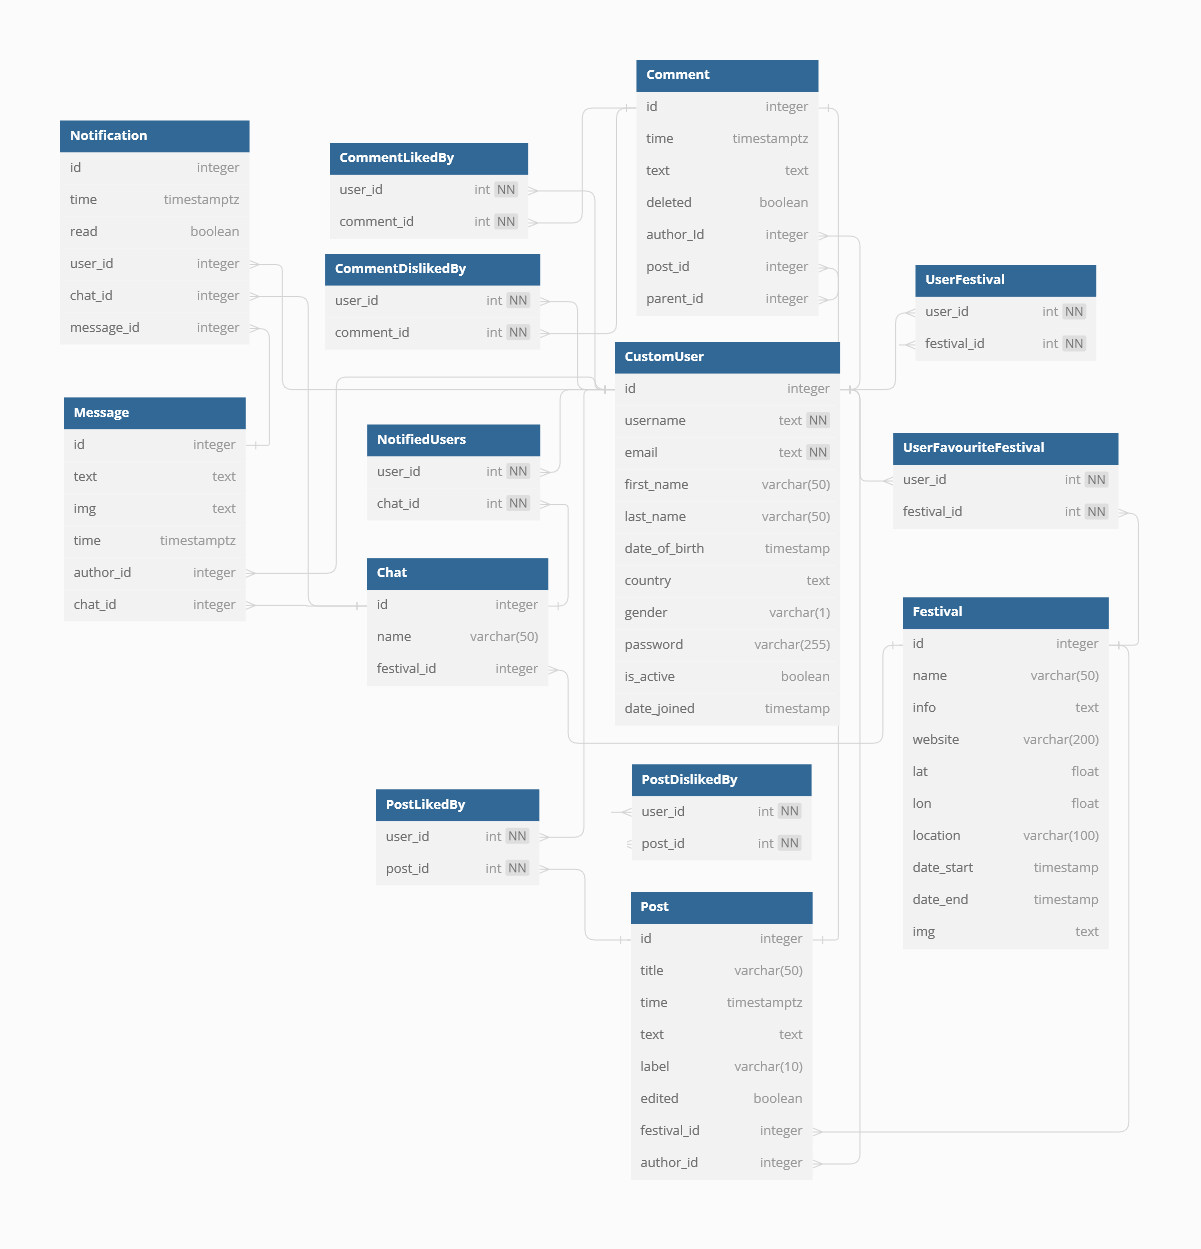
\includegraphics[width=\textwidth]{img/baza}
\end{center}
\caption{Podatkovni model razvite rešitve.}
\label{baza}
\end{figure}

\section{Zaledni del}
% - 1. na kratko kaj mamo u Djangu (views, models) in kaj v drf(serializers) in zakaj smo uporabili, ku funkcionira ORM
Za implementacijo zalednega dela smo uporabili Django v kombinaciji z Django REST Frameworkom.
Django nam je omogočil poenostavljeno delo s podatkovno bazo, saj nam z vgrajenim ORM sistemom, ni potrebno pisati SQL stavkov, temveč lahko kodiramo v Pythonu.
To naredi vsako interakcijo s podatkovno bazo lažjo in bolj intuitivno, istočasno pa ne rabimo skrbeti glede SQL napadov, saj ORM vsako poizvedbo sestavi s poudarkom na varnosti. 
Uporaba Django REST Frameworka pa nam je z orodji za serializacijo, avtentikacijo in generičnimi pogledi, še dodatno olajšala implementacijo REST APIja.

% - 2. primer modela, viewa in serializera in url, avtentikacijska pravila
\subsection{Delo s podatkovno bazo}
Uporaba Djanga nam je omogočila, da smo lahko enostavno ustvarili povezavo z zalednim delom aplikacije.
Najprej smo v datoteki \textit{models.py} definirali modele, ki v Djangu predstavljajo strukturo in relacije v podatkovni bazi s pomočjo objektov.
Vsak Django model predstavlja eno tabelo, vsako polje modela določeno kot atribut razreda, pa en stolpec v tabeli podatkovne baze.
Ko smo modele definirali, je Django poskrbel za kreacijo tabel glede na modele, vendar je bilo potrebno najprej pognati ukaz \textit{'python manage.py makemigrations'}, da so se ustvarile migracije.
Da smo spremembe v datoteki z migracijami dejansko uporabili in posodobili podatkovno bazo, pa je bilo potrebno pognati ukaz \textit{'python manage.py migrate'}.

Spodnja izvorna koda prikazuje, kako smo definirali model za \textit{Festival}.
Z opcijo \textit{blank} definiramo, da v zahtevku s čelnega dela ni potrebno navesti določenega polja.
Z \textit{null} pa definiramo, da je vrednost polja v podatkovni bazi lahko NULL.
Polje \textit{genre} služi kot povezava tipa mnogo-proti-ena na tabelo \textit{Genre} (en festival ima lahko več različnih žanrov).
Pri tem smo z \textit{models.SET\_NULL} določili, da se ob primeru izbrisa instance žanra v festivalih povezanih s tem žanrom polje \textit{genre} postavi na NULL.
Privzeta nastavitev je \textit{models.CASCADE}, ki bi v primeru, da je en žanr izbrisan, izbrisala vse festivale povezane s tem žanrom.
V razredu \textit{Meta} pa smo definirali, da so rezultati vsake poizvedbe privzeto urejeni po imenu festivala.

\begin{lstlisting}[label=code1,caption=Primer kreiranja modela Festival v Djangu.,frame=tb,captionpos=b]
class Festival(models.Model):
    name = models.CharField(max_length=50)
    info = models.TextField(
        blank=True, 
        default='No info provided'
    )
    website = models.URLField(
        blank=True,
        default='No website provided'
    )
    lat = models.FloatField(blank=True, null=True)
    lon = models.FloatField(blank=True, null=True)
    date_start = models.DateField(blank=True, null=True)
    date_end = models.DateField(blank=True, null=True)
    img = models.URLField(blank=True, null=True)
    
    genre = models.ForeignKey(
        Genre, 
        on_delete=models.SET_NULL, 
        null=True, 
        blank=True
    )

    class Meta:
        ordering = ['name']
\end{lstlisting}

\subsection{API}
Za komunikacijo čelnega dela aplikacije z zalednim delom, smo implementirali RESTful API s pomočjo Django REST Frameworka, ki na zahteve odjemalca posluša na vratih 8000.

Uporaba Django REST Frameworka je močno pospešila izgradnjo APIja, saj smo lahko na enostaven način definirali, katera polja modela bodo serializirana (pretvorjena iz zapletenih podatkovnih struktur v obliko JSON za lažji prenos).
Potrebno je bilo le definirati razred za vsak model, ter našteti katera polja bodo serializirana.
Poleg osnovnih polj lahko serializiramo tudi izpeljana polja, ki niso neposredno na voljo v modelu.
To lahko naredimo tako, da definiramo metodo za izračun vrednosti.
\begin{itemize}
    \item \textbf{is\_favourite} - Glede na uporabnika in izbrani festival, vrne vrednost \textit{True} ali \textit{False} odvisno od tega, ali ima uporabnik festival dodan med priljubljene.
    \item \textbf{get\_is\_mod} - Glede na uporabnika in izbrani festival, vrne vrednost \textit{True} ali \textit{False} odvisno od tega, ali je uporabnik moderator festivala.
    \item \textbf{get\_num\_favourites} - Glede na izbrani festival, vrne število vseh uporabnikov, ki imajo festival dodan med priljubljene.
\end{itemize}

\begin{lstlisting}[label=code2,caption=Primer serializacije podatkov za model Festival.,frame=tb,captionpos=b]
class FestivalSerializer(serializers.ModelSerializer):
    is_favourite = serializers.SerializerMethodField()
    is_mod = serializers.SerializerMethodField()
    num_favourites = serializers.SerializerMethodField()

    class Meta:
        model = Festival
        fields = ['id', 
                    'name', 
                    'info', 
                    'website', 
                    'lat', 
                    'lon',
                    'date_start',
                    'date_end',
                    'img',
                    'genre',
                    
                    'is_mod',
                    'is_favourite',
                    'num_favourites']
        
        def get_is_favourite(self, obj):
            user = self.context['request'].user
            return user in obj.favourite_by.all()
        
        def get_is_mod(self, obj):
            user = self.context['request'].user
            return user in obj.mods.all()
        
        def get_num_favourites(self, obj):
            return len(obj.favourite_by.all())
\end{lstlisting}

Poleg serializacije podatkov nam Django REST Framework omogoča tudi uporabo tako imenovanih generičnih pogledov (Generic Views).
Generični pogledi ponujajo pogosto uporabljene vzorce operacij CRUD in s tem poenostavijo proces grajenja APIja tako, da zmanjšajo potrebo po pisanju ponavljajoče kode.
Prav tako omogočajo uporabo vnaprej določenih razredov, ki omogočajo olajšano upravljanje s pravicami dostopa, iskanje in paginacijo.
V pogledu je potrebno tudi navesti, kateri razred naj se uporabi za serializacijo podatkov.
V spodnji kodi lahko vidimo primer generičnega pogleda \textit{ListCreateAPIView}, ki ponuja končne točke za operacije GET in POST.
Preko te končne točke smo dostopali do seznama vseh festivalov, pri čemer smo lahko uporabili filtriranje in iskanje ter dodajali nove festivale.
\begin{lstlisting}[label=code3,caption=Primer pogleda za model \textit{Festival}\, ki omogoča kreiranje\, iskanje in vračanje festivalov urejenih po popularnosti in datumu.,frame=tb,captionpos=b]
class FestivalList(generics.ListCreateAPIView):
    permission_classes = (IsAuthenticated,)
    serializer_class = FestivalSerializer
    filter_backends = [SearchFilter]
    search_fields = ['name']

    def perform_create(self, serializer):
        festival = serializer.save()
        festival.mods.add(self.request.user)

    def get_queryset(self):
        order_by = self.request.query_params.get('order')

        queryset = Festival.objects.all()
        user = self.request.user
        if order_by == 'Popularity':
            queryset = queryset.annotate(
                most_popular=Count('favourite_by')
                )
                .all()
                .order_by('-most_popular')
        else:
            queryset = queryset.order_by(
                F('date_start').desc(nulls_last=True)
            )
    ...
\end{lstlisting}

Po vsem tem smo morali definirati še URL končne točke za naš API.
To smo opravili v datoteki \textit{urls.py}, kjer smo za vsako točko definirami URL naslov ter pogled uporabljen za obdelavo zahtev.
Poleg končnih točk za avtentikacijo za katere je poskrbela knjižnica Djoser smo implementirali še 10 ostalih končnih točk:
\begin{itemize}
    \item festivals/
    \item festivals/\textless int:pk\textgreater
    \item festivals/\textless int:pk\textgreater/chats/
    \item festivals/\textless int:pk\textgreater/chats/\textless int:cpk\textgreater
    \item notifications/
    \item hotels/
    \item posts/
    \item posts/\textless int:pk\textgreater
    \item posts/\textless int:pk\textgreater/comments
    \item posts/\textless int:pk\textgreater/comments/\textless int:pk\textgreater
\end{itemize}

\subsection{Strgalnik}
Ena glavnih funkcionalnosti našega sistema je ta, da uporabniku omogoča prikaz preno\-čišč v bližini glasbenega festivala.
Za implementacijo smo morali najprej določiti, od kod bomo pridobivali podatke.
Najboljše bi to rešili, če bi obstajala storitev, ki bi ponujala brezplačen API za dostop do potrebnih podatkov, vendar se je izkazalo, da nobena ustrezna storitev tega ne ponuja.
Za dostop do APIjev storitev kot sta Booking.com in Airbnb~\cite{airbnbapi} je potrebnen dolgotrajen proces, po katerem dostop še vedno ni zagotovljen.
Zato smo se odločili, da bomo podatke strgali iz spletne strani Booking.com s pomočjo Python knjižnice BeautifulSoup4.
Ko uporabnik na čelni strani vnese parametre za iskanje, skripta na zalednem delu sestavi URL naslov, v taki obliki, kot če bi brskali po Bookingu, ter prebere vsebino strani in vrne rezultat nazaj odjemalcu.

\section{Implementacija Mapbox zemljevida}
Zemljevide smo v celoti implementirali na čelnem delu aplikacije s storitvijo Mapbox.
Za dostop do storitve smo ustvarili uporabniški račun, da smo pridobili žeton za dostop ter prenesli modul \textit{nuxt-mapbox}.
Nato smo ustvarili novo instanco zemljevida z začetnimi nastavitvami:
\begin{itemize}
    \item \textbf{container} - Referenca na HTML element, ki vsebuje zemljevid.
    \item \textbf{style} - Izbor predloge zemljevida. Izbrali smo predlogo Mapbox Streets, ki se osredotoča na prikaz cestišč.
    \item \textbf{center} - Geografske koordinate, ki bodo v začetku centrirane. V našem primeru te koordinate predstavljajo lokacijo prizorišča.
    \item \textbf{zoom} - Začetna povečava zemljevida. Izbrali smo stopnjo 16, saj omo-goča tako pregled nad prizoriščem, kot neposredno okolico.
\end{itemize}

Za osnovno delovanje Mapbox zemljevida v naši aplikaciji zadošča že nekaj vrstic kode:
\begin{lstlisting}[label=code4,caption=Primer kode za prikaz lokacije na Mapbox zemljevidu.,frame=tb,captionpos=b]
new mapboxgl.Map({
    container: 'map',
    style: 'mapbox://styles/mapbox/outdoors-v12',
    center: [lon, lat],
    zoom: 16
})

let el = document.createElement('div')
el.className = 'marker img1'
const marker = new mapboxgl.Marker(el)
    .setLngLat([lon, lat])
    .addTo(map)
\end{lstlisting}

Zanimivejša je implementacija iskanja poti do festivala.
Za to smo potrebovali Mapbox Directions API v kombinaciji z Mapbox Search Box vnosnim poljem.
Mapbox Directions API~\cite{mapboxdirections} nam je izračunal optimalne poti za vožnjo, ter nam vrnil podatke v obliki JSON z vsemi pripadajočimi koordinatami, časi, dolžinami in ostalimi metapodatki.
Mapbox Search Box pa nam je omogočil, da lahko uporabnik izbere izhodiščno lokacijo preko vnosnega polja v človeku prijaznem zapisu.

\subsection{Izbira izhodiščne lokacije}
Uporabnik lahko izhodiščno lokacijo izbere na 2 načina.
Prvi način je ta, da uporabnik preko vnosnega polja poišče lokacijo.
Ob izbiri lokacije, se sproži dogodek \textit{retrieve}, preko katerega lahko potem dostopamo do lokacije in izluščimo koordinate.

Druga opcija je, da uporabnik dovoli uporabo lokacije v aplikaciji.
S to izbiro, je za izris poti potem potreben le klik gumba.

Da smo pridobili podatke pa je bilo potrebno izvesti klic na Mapbox Directions API.
\begin{lstlisting}[label=code5,caption=URL za klic Mapbox Directions APIja\, ki vrne navodila za pot v formatu GeoJSON.,frame=tb,captionpos=b]
const response = $fetch(
    `https://api.mapbox.com/directions/v5/mapbox/driving/
    ${startLocation.lon}%2C${startLocation.lat}%3B
    ${props.lon}%2C${props.lat}?
    alternatives=false
    &geometries=geojson
    &language=en
    &overview=simplified
    &steps=true
    &access_token=${runtimeConfig.public.mapboxToken}`
)
\end{lstlisting}

Klic APIja vrne odgovor z navodili za vsak zavoj in vmesne točke, skupaj s pripadajočimi koordinatami.
Poleg tega dobimo tudi podatke o času trajanja vožnje v sekundah, ter dolžine poti v metrih.
Te podatke je potrebno nato še prikazati na zemljevidu.
\begin{lstlisting}[label=code6,caption=Izvorna koda za prikaz poti na zemljevidu.,frame=tb,captionpos=b]
map.on('load', () => {
    map.addSource('route', {
        'type': 'geojson',
        'data': {
            'type': 'Feature',
            'properties': {},
            'geometry': {
                'type': 'LineString',
                'coordinates': props.directions.geoLines
            }
        }
    });
    map.addLayer({
        'id': 'route',
        'type': 'line',
        'source': 'route',
        'layout': {
            'line-join': 'round',
            'line-cap': 'round'
        },
        'paint': {
            'line-color': '#26A69A',
            'line-width': 5,
        }
    })
})
\end{lstlisting}

Ko je pot prikazana na zemljevidu, je potem potrebno ponovno centrirati zemljevid tako, da je vidna celotna pot.
\begin{lstlisting}[label=code7,caption=Prilagoditev središča zemljevida in stopnje povečave\, da ustreza geografskemu območju poti.,frame=tb,captionpos=b]
const bounds = new mapboxgl.LngLatBounds()
props.directions.geoLines.forEach(([lon, lat]) => {
    bounds.extend([lon, lat])
})

const padding = { top: 50, bottom: 50, left: 50, right: 50 }
map.fitBounds(
    bounds,
    { padding }
)
\end{lstlisting}

\section{Realnočasovna komunikacija}
Pomembna stvar pri implementaciji klepetov je ta, da vsi uporabniki, ki so aktivni v določenem klepetu, takoj prejmejo novo sporočilo.
Prav tako morajo uporabniki, prijavljeni na obvestila za klepet nova obvestila prejeti takoj.
To smo dosegli z uporabo storitve Pusher Channels, ki sloni na tehnologiji WebSockets.
Kako smo to vključili v naš sistem pa bomo opisali v naslednjem poglavju.

Za delovanje Pusher Channels smo na zalednem delu najprej namestili knjižnico \textit{pusher}, na čelnem pa \textit{pusher-js}.
Nato smo ustvarili Pusher račun, da smo lahko pridobili pooblastila za uporabo Pusherja - \textit{app\_id, key in secret}.
Na zalednem delu smo nato ustvarili novo datoteko z Izvorno kodo~\ref{code8}, ki inicializira novo instanco Pusherja.
Podobno smo storili tudi na čelnem delu, kjer pa je bilo potrebno kot parameter podati le \textit{key}.
\begin{lstlisting}[label=code8,caption=Izvorna koda\, ki kreira novo instanco Pusherja na zalednem delu.,frame=tb,captionpos=b]
import pusher, os

pusher = pusher.Pusher(
    app_id=os.environ.get('PUSHER_APP_ID'),
    key=os.environ.get('PUSHER_KEY'),
    secret=os.environ.get('PUSHER_SECRET'),
    cluster='eu',
    ssl=False
)    
\end{lstlisting}

\subsection{Sporočila}
Najprej smo implementirali realnočasovno sporočanje.
Za začetek smo metodo \textit{perform\_create} v pogledu \textit{MessageList} prilagodili tako, da poleg kreiranja novega objekta, takoj odda sporočilo v kanal klepeta na Pusherju.
Potrebno je bilo podati ime kanala, ki smo ga poimenovali kar \textit{chat-'ime-klepeta'}, ime dogodka, ki smo ga poimenovali kar \textit{'new-message'}, ter vsebino samega sporočila.
\begin{lstlisting}[label=code9,caption=Pošiljanje novega sporočila vsem odjemalcem naročenim na kanal chat-{message.chat.id} z uporabo storitve Pusher.,frame=tb,captionpos=b]
data = serializer.data
pusher.trigger(
    f'chat-{message.chat.name}',
    'new-message',
    data
)
\end{lstlisting}

S tem smo pokrili zaledni del, implementirati pa je bilo potrebno še prejemanje teh sporočil na čelnem delu.
To smo naredili tako, da smo najprej ustvarili Nuxt vtičnik z instanco Pusherja.
Do tega vtičnika smo potem lahko dostopali preko celotne aplikacije in preprečili možnost, da bi brez potrebe kreirali več instanc Pusherja, kot bi jih potrebovali.
To nam je tudi omogočilo, da smo z eno instanco Pusherja upravljali tako nova sporočila, kot obvestila.

\begin{lstlisting}[label=code10,caption=Nuxt vtičnik za novo instanco Pusherja.,frame=tb,captionpos=b]
import Pusher from 'pusher-js'

export default defineNuxtPlugin(nuxtApp => {
    const pusher = new Pusher(
        runtimeConfig.public.pusherKey, {
            cluster: 'eu'
        })

    nuxtApp.provide('pusher', pusher)
})
\end{lstlisting}

Vse kar je preostalo je bila prijava na poslušanje novih sporočil.
Za to se je bilo potrebno naročiti na kanal za določen klepet, ter poslušati na dogodek \textit{'new-message'}, ter novo sporočilo na strani odjemalca dodati med obstoječa.

\begin{lstlisting}[label=code11,caption=Poslušanje na nova sporočila na čelnem delu.,frame=tb,captionpos=b]
const channel = useNuxtApp().$pusher.subscribe(
    `chat-${chatName}`
)       
channel.bind('new-message', (data) => {
    apiMessages.value.push(data)
})
\end{lstlisting}

\subsection{Notifikacije}
Podobno kot smo implementirali prejemanje sporočil v realnem času, smo implementirali tudi obvestila.
Razlika je bila le ta, da smo na zalednem delu najprej iterirali čez vse klepete za katere ima uporabnik vklopljena obvestila, in se za vsakega posebej naročili na nov kanal.

\section{Večnivojski komentarji}
Implementacija foruma, je bila časovno najbolj potratna, zaradi velikega števila funkcionalnosti, ki jih podpira.
Za delovanje foruma smo v Djangu potrebovali modele \textit{CustomUser}, \textit{Festival}, \textit{Post} in \textit{Comment}, ter vse potrebne vmesne modele za všečkanje objav in komentarjev.

Največji izziv pri implementaciji foruma je bil, kako omogočiti gnezdenje komentarjev.
V sistemu, ki omogoča gnezdenje komentarjev, lahko uporabnik odgovori na predhodnje komentarje, pri čemer se ustvarja hierarhija komentarjev.
Prednost tega pristopa je predvsem lažja berljivost, saj se s tem izognemo zmedi kateremu komentarju pripada odgovor.

Za hranjenje hierarhije komentarjev smo na zalednem delu definirali model \textit{Comment} in uporabili samoreferenčni tuji ključ.
To storimo tako, kot kadar definiramo relacije mnogo proti ena, le da za referenco uporabimo kar besedo \textit{'self'}~\cite{djangoselfreference}.
S tem smo dosegli, da ima lahko en komentar enega samega starša in več odgovorov, starš pa je lahko tudi \textit{null}, kar definira komentarje na najvišjem nivoju.
\begin{lstlisting}[label=code12,caption=Definiranje hierarhije komentarjev v modelu Comment z uporabo samoreferenčnega tujega ključa.,frame=tb,captionpos=b]
parent = models.ForeignKey(
    'self',
    null=True,
    blank=True,
    related_name='child_comments',
    on_delete=models.CASCADE
)
\end{lstlisting}

Potem je bilo potrebno poskrbeti še za ustrezno serializacijo podatkov, za kar smo napisali rekurzivno metodo \textit{get\_child\_comments}, ki za določen komentar zbere vse pripadajoče odgovore in jih sestavi v formatu JSON za prenos do odjemalca.
\begin{lstlisting}[label=code13,caption=Rekurzivna metoda za serializacijo komentarjev v obliki nadrejen/podrejen.,frame=tb,captionpos=b]
def get_child_comments(self, obj):
    child_comments = obj.child_comments.all()
    return CommentSerializer(
        child_comments,
        context=self.context,
        many=True
    ).data
\end{lstlisting}

Potem pa še ustrezen pogled, ki ob klicu na končno točko vrne vse komentarje na najvišjem nivoju skupaj z pripadajočimi odgovori.
\begin{lstlisting}[label=code14,caption=Pogled\, ki s filtriranjem izbere samo komentarje na najvišjem nivoju.,frame=tb,captionpos=b]
class CommentList(generics.ListCreateAPIView):
    serializer_class = CommentSerializer

    def get_queryset(self):
        post = self.kwargs['pk']
        return Comment.objects.filter(
            post=post, 
            parent__isnull=True
        )
\end{lstlisting}

Nato je bilo potrebno komentarje prikazati še na strani odjemalca, kjer smo ustvarili rekurzivno komponento \textit{Comment}.
Za prikaz odgovorov na komentarje ter zamik na vsakem nivoju, smo uporabili spremenljivko \textit{level}, ki smo jo podali kot parameter rekurzije.
\begin{lstlisting}[label=code15,caption=Rekurzivna komponenta za prikaz komentarjev na strani odjemalca.,frame=tb,captionpos=b]
<div 
    v-if="comment.child_comments
    && comment.child_comments.length
    && showReplies"
>
    <Comment
        v-for="(childComment, childIndex)
            in comment.child_comments"
        :key="childComment.id"
        :index="childIndex"
        :comment="childComment"
        :level="level + 1"
    />
</div>
\end{lstlisting}

Ostala implementacija je bila dokaj preprosta.
Po tem, ko smo omogočili komentiranje, smo dodali še možnosti iskanja in urejanja komentarjev po času, ter po številu všečkov.
Implementirali pa smo tudi paginacijo, da smo velike množice podatkov lahko razbili na manjše dele in jih na bolj učinkovit poslali do odjemalca.

\section{Firebase}
Za shranjevanje slik smo uporabili Firebase Storage, ker omogoča varno ter enostavno shranjevanje in branje datotek in lahko integracijo v aplikacijo.
Enako kot pri Mapboxu ter Pusherju se je bilo najprej potrebno registrirati, da smo dobili vse potrebne žetone.
Potem smo ustvarili nov Nuxt vtičnik, ki hrani instanco Firebasa, da lahko do njega dostopamo v katerem koli delu aplikacije.

Sliko smo v Firebase Storage shranili tako, da smo najprej definirali pot, kjer bo slika shranjena v oblaku, ter referenco do te shrambe.
Da ne bi prišlo do nepotrebnih težav, je bilo potrebno poskrbeti, da se nobeno ime slike ne ponovi.
To smo rešili tako, da smo vsako sliko poimenovali z imenom slike in trenutnim časom v milisekundah.
Potem smo z uporabo metode \textit{uploadBytes} naložili sliko v shrambo.
V primeru, ko se slika uspešno shrani, dobimo nazaj URL naslov za prenos datoteke.
Ta URL naslov smo potem shranili v našo podatkovno bazo, da smo lahko v aplikaciji dostopali do slike.
\begin{lstlisting}[label=code16,caption=Nuxt vtičnik za shranjevanje slik z uporabo Firebase Storage.,frame=tb,captionpos=b]
const uploadImage = async() => {
    const storage = useNuxtApp().$storage
    const fileName = `festival-themes/
        ${Date.now()}-${festival.value.img.name}`
    const imageRef = storageRef(storage, fileName)

    try {
        await uploadBytes(imageRef, festival.value.img)
        const url = await getDownloadURL(imageRef)
        return url 
    }
    catch (error) {
        console.log("Error uploading image")
    }
}
\end{lstlisting}

\chapter{Predstavitev aplikacije}
V naslednjem poglavju smo predstavili razvito aplikacijo z vidika uporabnika.
Opisali smo funkcionalnosti, ki jih uporabniški vmesnik omogoča, pri čemer smo si pomagali s slikami.

\section{Uporabniški vmesnik}
\label{UI}
Uporabniški vmesnik aplikacije je sestavljen iz štirih glavnih strani.
To so domača začetna stran, stran za vsak festival ter pripadajoči forum in klepeti.
Poleg teh strani aplikacija vsebuje še strani za dodajanje in urejanje festivalov, objav in klepetov, ter registracijo in prijavo.
Vse strani (razen registracije in prijave) vsebujejo še orodno vrstico, preko katere se lahko uporabniki odjavijo iz aplikacije ter dostopajo do obvestil, foruma in domače strani.

\subsection{Domača stran}
Domača stran je namenjena temu, da lahko uporabniki najdejo glasbene festivale in dodajo nove.
Za lažje iskanje uporabniku relevantnih festivalov, smo implementirali naslednje možnosti iskanja in filtriranja:
\begin{itemize}
    \item Iskalno okno, preko katerega lahko iščejo po imenu festivala ter lokaciji.
    \item Spustni seznam preko katerega lahko uredijo izpis po datumu in popularnosti.
    \item Omejitev časovnega obdobja v katerem poteka festival.
    \item Izpis samo prihajajočih dogodkov.
    \item Izpis samo uporabnikovih priljubljenih festivalov.
\end{itemize}

Rezultati iskanja so prikazani na karticah, in vsebujejo ime, lokacijo in datume festivala.
Če je na voljo, se prikaže tudi slika festivala.
V levem zgornjem kotu kartice je za vsak festival prikazano, koliko uporabnikov ima festival dodan med priljubljene.
V spodnjem desnem kotu lahko uporabnik razširi kartico, in s tem prikaže še podrobnejši opis.
S klikom na gumb 'EXPLORE' v spodnjem levem kotu, pa se odpre stran za izbrani festival.

\begin{figure}[htb] % OPTIONS h-here, t-top, b-bottom, p-page
    \begin{center}
        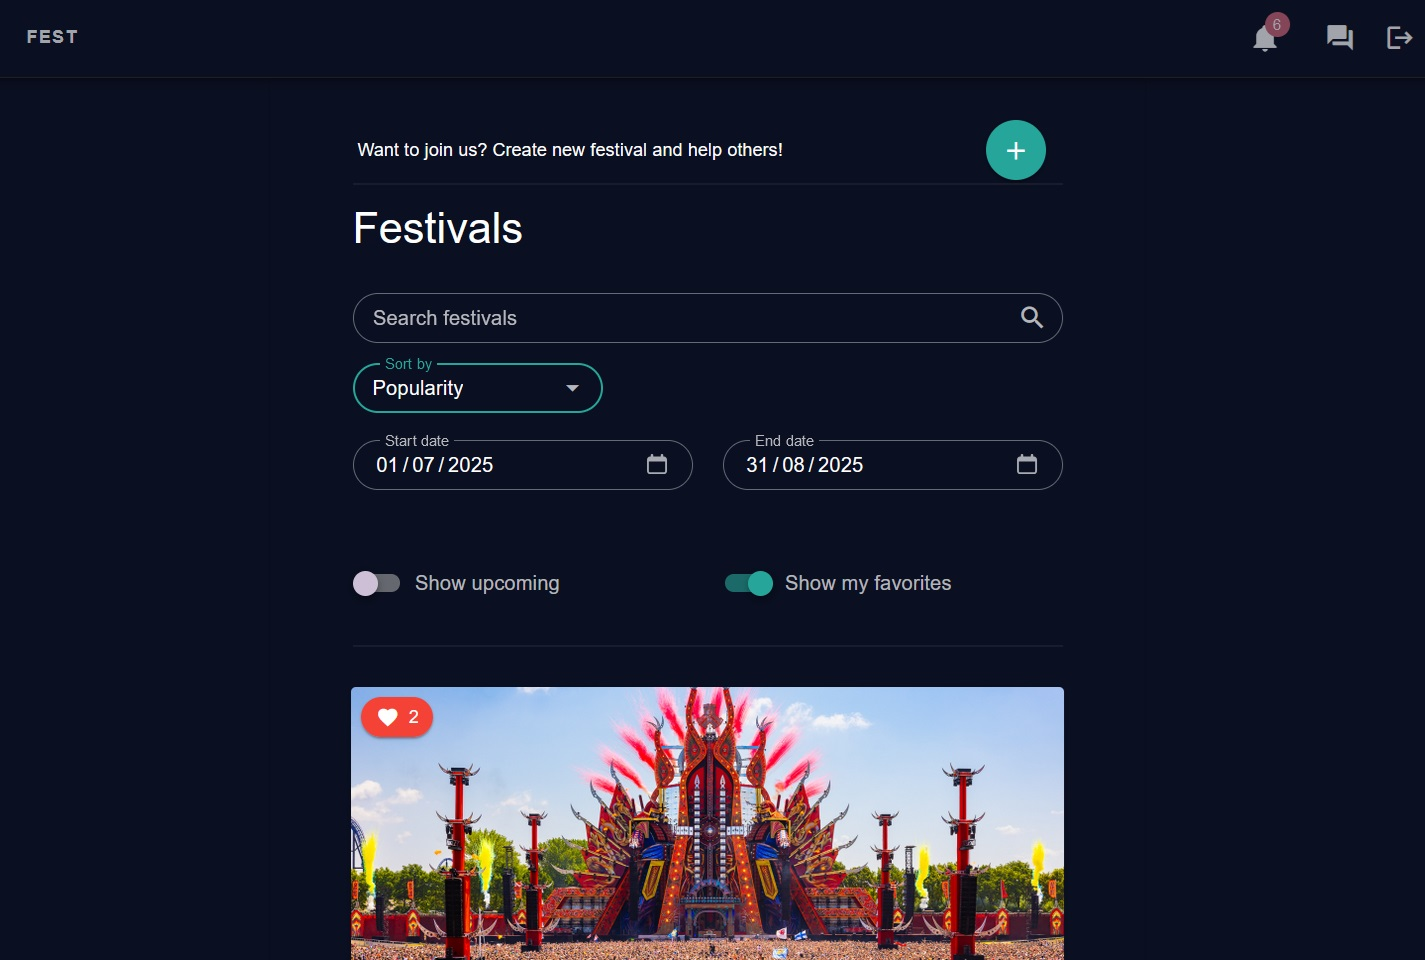
\includegraphics[width=0.99\textwidth]{img/homepage}
    \end{center}
    \caption{Domača stran spletne aplikacije.}
    \label{homepage}
\end{figure}

\begin{figure}[htb] % OPTIONS h-here, t-top, b-bottom, p-page
    \begin{center}
        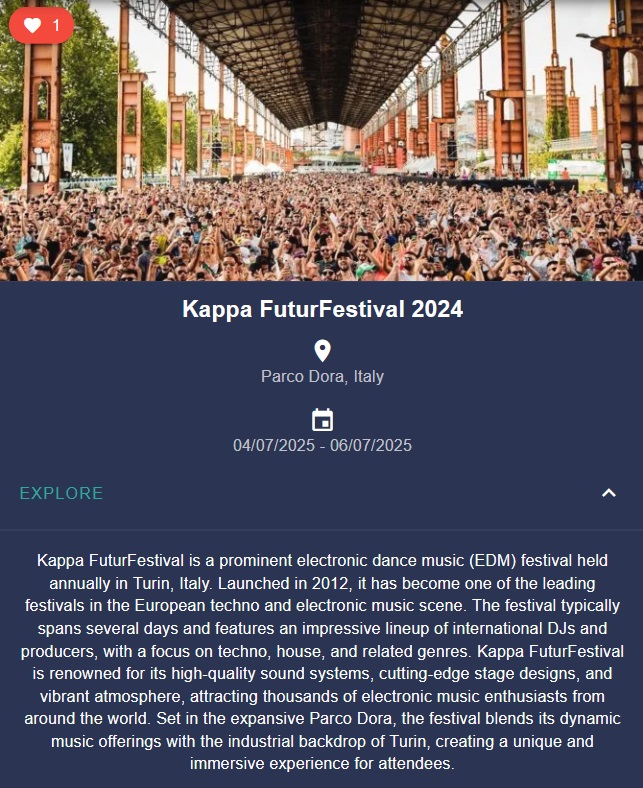
\includegraphics[width=0.7\textwidth]{img/homepagecard}
    \end{center}
    \caption{Kartica za festival na domači strani.}
    \label{homepage}
\end{figure}

Poleg iskanja začetna stran omogoča tudi dodajanje novega festivala.
S klikom na gumb z oznako +, se odpre novo okno z obrazcem.
Tu uporabnik vnese vse potrebne podatke, vključno z lokacijo, katero lahko vnese preko zemljevida.

Festivale lahko v sistem zaenkrat dodajo vsi uporabniki, kar omogoča lažjo pridobitev manjših in manj poznanih festivalov.
Uporabnik, ki doda festival avtomatsko postane moderator tega festivala.
To mu omogoča, da lahko ureja stran festivala in vse pripadajoče forume.
V prihodnosti bi bilo smiselno dodati tudi možnost uradnih partnerjev.
Tako bi lahko organizatorji glasbenih festivalov stopili v kontakt z nami, šli čez določen proces in postali partnerji, s čimer bi aplikacija pridobila točnejše informacije in morebitno dodatno vsebino, ki bi lahko še okrepila uporabniško izkušnjo.

\section{Festivalska stran}
Na festivalski strani so prikazane podrobnosti določenega festivala.
Uporabnik lahko tu najde informacije o lokaciji (z zemljevidom), žanrih, datumih, uradni spletni strani in ostalem.
Od tu dobi tudi povezavo do foruma in klepetov za izbrani festival.
Za boljšo uporabniško izkušnjo in kompletno rešitev, pa lahko uporabnik razširi zavihek 'Sleeping options and directions', kjer lahko poišče prenočišča v bližini, ter navodila za pot do festivala.

\subsection{Prenočišča v bližini}
V primeru, da uporabnik izbere možnost iskanja prenočišč v bližini glasbenega festivala, se odpre okno preko katerega lahko vnese različne parametre za iskanje.
Izbere lahko število ljudi, število sob, datum prijave, datum odjave in najvišjo ceno prenočišča na noč.
Določi pa lahko tudi kateri rezultati se prikažejo prvi, pri čemer lahko izbira med najcenejši najprej, najbolje ocenjeni naprej, najbolje ocenjeni z nizko ceno najprej, ter najkrajša pot do festivala najprej.
Datumi prijave in odjave so privzeto nastavljeni na prvi in zadnji dan festivala, po tem pa lahko uporabnik poljubno podaljša ali skrajša termin.
V primeru da festival že poteka, je uporabnik o tem tudi obveščen, datum prijave pa postane tekoči dan.
Tudi v primeru da novi datumi za festival še niso določeni, lahko uporabnik poišče prenočišča, datum prijave postane tekoči dan, datum odjave pa 3 dni za tem.

Rezultati poizvedbe so prikazani na karticah, na katerih za vsako pre-nočišče najdemo podatke o imenu prenočišča, ceni na noč, kraju, povprečni oceni in številu ocen, ter oddaljenosti od prizorišča festivala.
S klikom na gumb 'DETAILS', je uporabnik preusmerjen na stran prenočišča na Bookingu.

\subsection{Navodila za pot}
Uporabnik lahko pridobi tudi navodila za pot do glasbenega festivala.
Za izbor začetne lokacije ima na voljo dve možnosti.
Prva je ta, da vnese lokacijo preko vnosnega polja, pri čemer se mu lokacije ob vnosu teksta avtomatsko predlagajo.
Druga možnost pa je, da uporabnik dovoli aplikaciji dostop do lokacije.
S to možnostjo se prikaže gumb, s katerim lahko uporabnik zahteva navodila za pot s svoje trenutne lokacije.

Po izboru ene izmed teh možnosti, se zemljevid z lokacijo festivala posodobi v zemljevid s potjo od izbrane lokacije do prizorišča.
V levem zgornjem kotu se izpiše čas trajanja vožnje in dolžina v kilometrih, nad zemljevidom pa se izpišejo podrobna navodila za pot.

\section{Forum}
Forum je namenjen temu, da uporabniki delijo novice, mnenja in nasvete, lahko pa tudi postavijo vprašanja glede stvari, ki jih zanimajo oz. jim niso jasna.
S tem jim omogočimo, da se povežejo in sodelujejo, ter si pri tem pomagajo.
Kar pa je najpomembneje je to, da na ta način uporabniki dobijo mnenja ostalih uporabnikov.
Takšna mnenja največ štejejo, saj lahko tisti, ki so že obiskali festival podajo največ praktičnih nasvetov.

\subsection{Objave}
Vsaka objava je predstavljena na kartici, ki je ločena na 2 dela.

Zgornji levi del kartice vsebuje informacije o festivalu, času objave, lastniku objave, ter tipu objave.
Zgornji desni del kartice pa vsebuje meni, ki omogoča brisanje (lastnik in moderator) in urejanje (lastnik) objav.

Spodnji del kartice vsebuje naslov in vsebino objave, pod njima pa najdemo še gumba za všečkanje in nevšečkanje, ter gumb za dostop do komentarjev, ki odpre objavo na novi strani.
Vsi gumbi vsebujejo tudi podatke o številu všečkov in nevšečkov, ter številu komentarjev za objavo.

Uporabnik lahko tudi brska po objavah.
To mu omogoča iskalno polje preko katerega lahko išče objave po naslovu, vsebini in uporabniku.
Na voljo so tudi filtri za določen tip objave, zato da lahko uporabnik izbere samo kategorijo objav, ki ga v trenutku zanima.
Rezultate je mogoče razvrstiti po naslednjih kriterijih:
\begin{itemize}
    \item \textbf{Top} - Največje število všečkov
    \item \textbf{Most commented} - Največje število komentarjev
    \item \textbf{Best} - Najboljše razmerje med všečki in nevšečki
    \item \textbf{New} - Najnovejši na začetku
    \item \textbf{Controversial} - Urejeni tako, da so na vrhu prikazane tiste objave, ki imajo razmerje všečkov in nevšečkov približno 1:1
\end{itemize}
Razvrstitev objav po kontroverznosti je lahko uporabniku v pomoč, saj niso vsa mnenja vseh ljudi vedno enaka.
Morda bo nekomu neka informacija koristila, nekomu pa ne.

\subsection{Komentarji}
Komentarji so ključni del foruma, saj omogočajo, da vsi uporabniki podajo svoje mnenje na objavo.
Brez komentarjev, bi bila komunikacija le enostranska in posledično ne bi bila v veliko pomoč.

Komentarje za objavo dosežemo tako, da kliknemo na izbrano objavo.
Po izbiri objave, se objava v isti obliki odpre na novi strani.
Pod objavo je tekstovno polje, ki se ob kliku spremeni v besedilno polje, preko katerega lahko uporabnik doda komentar, ter spustni seznam, preko katerega lahko uporabnik razvrsti komentarje po novejših ali pa priljubljenejših najprej.
Sledijo vsi komentarji, ki pripadajo objavi.

Komentarji so prikazani podobno kot objave, le da zgornji del kartice vsebuje samo ime uporabnika in čas objave.
Spodnji del vsebuje vsebino komentarja, všečke in nevšečke, ter gumb s katerim lahko uporabnik odgovori na komentar.

Kot smo že omenili so komentarji prikazani večnivojsko.
Vsak odgovor na komentar je na zaslonu zamaknjen za nekaj pikslov v desno, kar uporabniku omogoča lažji pregled, še posebej v primerih, ko je pod objavo veliko število komentarjev.
Privzeto sta prikazana samo prva dva nivoja komentarjev, sepravi vsi korenski komentarji vključno z odgovori.
S pomočjo gumba pod komentarji, ki vsebujejo odgovore pa lahko naknadno uporabnik skrije ali prikaže komentarje.

\section{Klepetalnica}
Klepetalnica je namenjena temu, da se uporabniki lahko povežejo med sabo.
Vsak festival ima svojo pripadajočo klepetalnico, v kateri lahko uporabniki razpravljajo v živo.
Tu imajo uporabniki odprte roke pri uporabi, ker so javne pa se lahko klepetom pridruži vsak.
Tako lahko uporabniki med drugim:
\begin{itemize}
    \item Ustvarijo klepet, v katerem se zberejo uporabniki aplikacije iz neke države.
    \item Tisti, ki potujejo sami lahko ustvarijo klepet z namenom, da najdejo ljudi za skupni obisk in planirajo srečanja.
    \item Med potekom festivala lahko razpravljajo o novicah ali pa novostih in spremembah glede na prejšnja leta.
    \item Z ostalimi delijo informacije o tem, kje lahko najdejo različne stojnice s hrano in pijačo, kje lahko prevzamejo festivalske zapestnice ipd.
    \item Razpravljajo o nastopajočih ali pa delijo vtise iz prejšnjih dni.
\end{itemize}

\subsection{Klepet}
Do klepetov lahko uporabnik dostopa preko strani izbranega festivala, kjer najprej vidi seznam vseh obstoječih klepetov.
Potem lahko izbira med dodajanjem novega klepeta, ali uporabe že obstoječega.

Vsak klepet je zgrajen iz:
\begin{itemize}
    \item Naslovne vrstice z imenom klepeta in gumbom za prijavo/odjavo na obvestila.
    \item Okna kjer so prikazana vsa sporočila.
    \item Vrstice z vnosnim poljem in gumbom za pošiljanje sporočil.
\end{itemize}
% insert slika chata

Okno, kjer so prikazana vsa sporočila v klepetu je sestavljeno tako, da je razvidno komu sporočilo pripada.
Uporabnik vidi svoja sporočila poravnana na desno stran klepeta, sporočila ostalih pa so poravnana na levo, skupaj z ikono, ki predstavlja uporabnika.
Sporočila so lahko tekstovna ali pa slikovna.
Nad vsakim sporočilom poslanim po daljšem obdobju od prejšnjega, izpiše, kdaj je bilo sporočilo poslano.
Uporabnik lahko pošlje tekstovno ali slikovno sporočilo, lahko pa tudi oboje hkrati.
Ob kliku na tekstovno sporočilo se poleg sporočila prikažeta točen datum in ura ob katerem je bilo sporočilo poslano.
Klik na sliko, pa odpre sliko čez celoten zaslon, hkrati pa se na dnu slike izpišeta ime slike ter datum in ura sporočila.
Če sporočilo vsebuje tako tekst kot sliko, je prikaz isti kot pri slikovnih sporočilih, le da se pod sliko izpiše še tekst.

Sporočila se prenašajo realnočasovno, se pravi, da so uporabnikom na voljo takoj ko so poslana.
Ko je v klepet dodano novo sporočilo, ali pa se uporabnik pomakne v klepetu navzgor, se na dnu klepeta prikaže gumb, ki mu omogoči da se vrne nazaj na dno klepeta.

Za nova sporočila je na dnu zaslona uporabniku na voljo vrstica sestavljena iz gumba za izbiro datoteke, tekstovnega polja in gumba za pošiljanje.
Gumb za pošiljanje je onemogočen dokler ni izbrana slika ali pa je vpisan tekst.


\subsection{Obvestila}
Pomemben del klepetov so tudi obvestila, ki se prav tako kot pošiljanje sporočil osvežujejo v realnem času.
Uporabnik se lahko poljubno prijavi (in odjavi) na obvestila za klepete katerim želi slediti tako, da v naslovni vrstici klepeta klikne na ikono s sliko zvonca, zraven katerega piše tudi število klepetov z novimi obvestili.
Obvestilo o novem sporočilu prejmejo vsi uporabniki razen pošiljatelja.
Do novih obvestil lahko dostopamo preko ikone z zvoncem v orodni vrstici aplikacije.
Za vsak klepet kjer obstaja novo obvestilo, se izpiše ime klepeta ter čas prejetega obvestila. 
Prejetih obvestil za en klepet je lahko več, zato se poleg že omenjenega izpiše tudi podatek o številu novih sporočil.
S klikom na obvestilo, se odpre klepet, nad zadnjim prebranim sporočilom pa tekst, ki obvešča katero sporočilo je bilo nazadnje prebrano.

\chapter{Zaključek}
V diplomski nalogi smo predstavili razvoj spletne aplikacije za glasbene festivale.
Cilj aplikacije je bil uporabnikom olajšati iskanje informacij povezanih s festivali in ustvariti omrežje, v katerem si lahko uporabniki pomagajo med sabo.
To nam je tudi uspelo, saj smo z implementacijo uporabnikom ponudili rešitev, ki jim poleg iskanja glasbenih festivalov omogoča tudi lažje planiranje, ter komunikacijo z ostalimi uporabniki.
Pri tem lahko med festivali izbirajo s pomočjo različnih filtrov, za vsak festival pa lahko poiščejo prenočišča v bližini ter navodila za pot.
Istočasno jim sistem omogoča, da preko foruma postavljajo vprašanja in delijo nasvete ter novice.
Preko klepetov pa lahko z ostalimi komunicirajo v realnem času, se morda dogovorijo za skupni obisk festivala, ali pa se pogovarjajo med samim festivalom ter tako popestrijo festivalsko izkušnjo.
Implementirali smo tudi obvestila, s čimer smo uporabniku omogočili, da je na tekočem z vsemi klepeti katerim želi slediti.
Pomembno je tudi to da smo razvili uporabniški vmesnik, ki je intuitiven in enostaven za uporabo, njegova odzivnost pa omogoča, da se lepo prikaže na napravah vseh velikosti.

Ideja za aplikacijo izhaja iz mojih slabih izkušenj obiskov glasbenih festivalov, saj sem večkrat naletel na težave, ki jih najverjetneje ne bi nikoli imel, če bi obstajala platforma kjer bi lahko uporabniki delili svoje pretekle izkušnje in nasvete z ostalimi.
Poleg tega je vedno potrebno iskati prenočišča v bližini festivala, za kar je potrebno uporabiti enega izmed spletnih ponudnikov prenočišč ter pri tem iskati najprej lokacijo, ter nato datume, za kar naša rešitev poskrbi sama.
Potrebno je le vnesti število potujočih in z enim klikom pridobiti prenočišča.

Ta aplikacija je bila moj prvi večji projekt, ki sem se ga sam lotil v času študija.
Kljub začetnim problemom in ne prav dobri seznanjenosti z nekaterimi tehnologijami, je razvoj potekal iz dneva v dan boljše.
Odnesel sem veliko novega znanja tako pri načrtovanju, kot razvoju čelnega in zalednega dela, ter uporabe orodij za kontejnerizacijo in upravljanje različic.
Prepričan sem, da mi bo znanje ki sem ga pridobil dobro služilo tudi v prihodnosti.

\section{Možnosti nadaljnjega razvoja}
Aplikacija, ki smo jo razvili je že precej obsežna, še vedno pa nudi veliko možnosti za nadaljnji razvoj.
Nekaj teh možnosti bomo našteli v nadeljevanju.

\subsection{Uradni partnerji}
Aplikacija že sedaj vsem uporabnikom omogoča dodajanje novih festivalov, bi pa to lahko nadgradili tako, da bi se povezali z organizatorji festivalov.
S tem bi lahko uporabniki med drugim pridobili predhodni dostop do vstopnic in nastopajočih, ali pa interaktivne zemljevide, ki jih nekateri organizatorji ponujajo.
Seveda bi lahko organizatorji z ostalimi delili tudi vse pomembne novosti in novice.
Tako bi lahko organizatorji festivalov upravljali svoj festival na naši rešitvi, istočasno pa bi jih naša rešitev reklamirala.
Težava, ki bi se pri tem lahko pojavila je ta, da organizatorji ne bi želeli sodelovati zaradi morebitnih kritik na svoj račun s strani uporabnikov.

\subsection{Klepeti}
Možnosti za nadgradnjo klepetov je kar nekaj.
Najbolj očitna možnost, ki se nam ponuja je implementacija potisnih obvestil.
Obvestila smo v našem sistemu že implementirali, bi jih pa lahko še nadgradili.
Ta bi največ doprinesla tistim, ki bi aplikacijo uporabljali na mobilnih napravah in izboljšala uporabniško izkušnjo predvsem v primerih, ko bi uporabniki klepete uporabljali na prizorišču.

Poleg tega v sistemu trenutno ni možno vedeti, kdaj je bil uporabnik nazadnje aktiven v aplikaciji.
S tem, da bi beležili aktivnost uporabnika, bi uporabnikom dalo vpogled v razpoložljivost osebe v klepetu.

\subsection{Zemljevidi}
Zemljevidi sedaj omogočajo iskanje poti in navodila za pot.
Te bi bilo mogoče nadgraditi tako, da bi uporabniku ponudili več možnih poti do prizorišča med katerimi bi lahko izbiral.
Smiselno bi bilo dodati tudi način javnega prevoza, vendar na žalost Mapbox te opcije ne ponuja.

%\cleardoublepage
%\addcontentsline{toc}{chapter}{Literatura}

% če imaš težave poravnati desni rob bibliografije, potem odkomentiraj spodnjo vrstico
\raggedright

\printbibliography[heading=bibintoc,type=article,title={Članki v revijah}]

\printbibliography[heading=bibintoc,type=inproceedings,title={Članki v zbornikih}]

\printbibliography[heading=bibintoc,type=incollection,title={Poglavja v knjigah}]

% v zadnji verziji diplomskega dela običajno združiš vse tri vrste referenc v en sam seznam in
% izpustiš delne sezname
\printbibliography[heading=bibintoc,title={Literatura}]

\end{document}

